\subsection{Preliminaries}
\label{sec:preliminaries}

In this Section, we provide some background information that is used in our proposed methods for geolocated time series summarization. Initially, we define {\em geolocated time series} followed by distance measures that we use in the spatial and time series domain. Then we describe the \isax family of trees \cite{shieh2008kdd,camerra2010icdm,camerra2014kais}, which can only index the {\em time series} information of each object, as well as the {\em hybrid} \btsr \cite{chatzig17btsr}. The latter is essentially an R-tree, built on the spatial locations of the times series, but additionally summarizing in each node the time series contained in the respective subtree. Finally, we briefly present the {\em tile maps} visual summarization method, indicating the concentration of a dataset in specific parts of its feature domain and the {\em timebox}, which is essentially a rectangle in the time series domain.

\subsubsection{Geolocated Time Series}
\label{subsec:geoTS}
A {\em time series} is a time-ordered sequence of values $T = \{v_1, \ldots, \\v_w\}$, where $v_i$ is the value at the $i$-th time point and $w$ is the length of the series. In this work, we deal with time series that are additionally characterized by a \emph{location}, denoted by $T.loc$, namely {\em geolocated time series}~\cite{chatzig17btsr}. Assuming a 2-dimensional space, we further use the notation $T.loc_x$, $T.loc_y$ to refer to the $(x,y)$ coordinates of $T$'s location. 

\subsubsection{Distance Measures}
\label{subsec:dist_meas}
The following distance measures are used, either in building, or when traversing the indices to generate the geolocated time series summaries.

\paragraph{Spatial Distance} In the {\em spatial domain}, the distance between two geolocated time series $T$ and $T'$ of equal length $w$ is calculated using the Euclidean distance of their respective locations. Furthermore, we normalize this distance with $maxDist_{sp}$, i.e., the maximum spatial distance of any pair of objects in the dataset, to obtain a measure in the interval $[0,1]$. Thus:

\begin{equation} \label{eq:dist_sp}
dist_{sp}(T, T') = \frac{\sqrt{(T.loc_x - T'.loc_x)^2 + (T.loc_y - T'.loc_y)^2}}{maxDist_{sp}}
\end{equation} \label{eq:2}

\paragraph{Time Series Distance} In the {\em time series domain}, similarly to other prior works (e.g., \cite{shieh2008kdd}), we also apply the Euclidean distance to measure the similarity of a pair of objects. In future work, we plan to make use of more complex distance measures \cite{paparrizos2015k}. More specifically, we calculate the distance between two time series $T$ and $T'$ as follows:

\begin{equation} \label{eq:dist_ts}
dist_{ts}(T, T') = \frac{\sqrt{\displaystyle \sum_{i=1}^{w}(v_i - v'_i)^2}}{maxDist_{ts}}
\end{equation}

\noindent where $maxDist_{ts}$ denotes the maximum distance of any pair of objects in the dataset and is used for normalization, as above.

\subsubsection{SAX Representation of Time Series}
\label{subsec:sax}

The {\em Symbolic Aggregate approXimation (SAX)} is a multi-resolution representation of a time series introduced in \cite{shieh2008kdd}. It can be derived from its {\em Piecewise Aggregate Approximation} (PAA) \cite{keogh2001paa,faloutsos2000vldb} by quantizing the PAA segments on the $v$-axis. As exemplified in Figure~\ref{fig:isax_representation}, a time series $T_2$ is transformed to a PAA representation of $w$=3 words with real-valued coefficients (the horizontal red bars). To get a $SAX$ representation for a time series, these coefficients are discretized along the $v$-axis using {\em breakpoints} (shown with dashed lines) assuming a $\mathcal{N}(0,1)$ Gaussian distribution that enables generation of equi-probable symbols for a given cardinality ($b=4$ symbols are used in this example). Interestingly, by using bitwise representations for these symbols, coarser $SAX$ values can be obtained from more refined ones, by simply ignoring trailing bits. Importantly, the Euclidean distance between $SAX$ representations of two time series is guaranteed to be a {\em lower bound} with respect to the Euclidean distance over the original time series. Formally, for two time series $T, T'$ of equal length $n$ using their respective $SAX$ words $T_w, T'_w$ of size $w$, it holds that:

\begin{equation} \label{eq:dist_sax}
d_{SAX}(T_w, T'_w) =\sqrt{\frac{n}{w}} \sqrt{\sum_{j=1}^{w} d^2 (t_j, t'_j) }  \leq {\sqrt{\displaystyle \sum_{i=1}^{n}(T.v_i - T'.v_i)^2}}
\end{equation}

\noindent where $d(t_j, t'_j)$ is the distance between symbols at the $j$-th position of each $SAX$ word. Comparisons between \isax words of different cardinality are possible by promoting the \isax representation of lower cardinality to the cardinality of the larger, as the lower bound in Eq.~\ref{eq:dist_sax} still holds.

\begin{figure}[t]
	\centering
	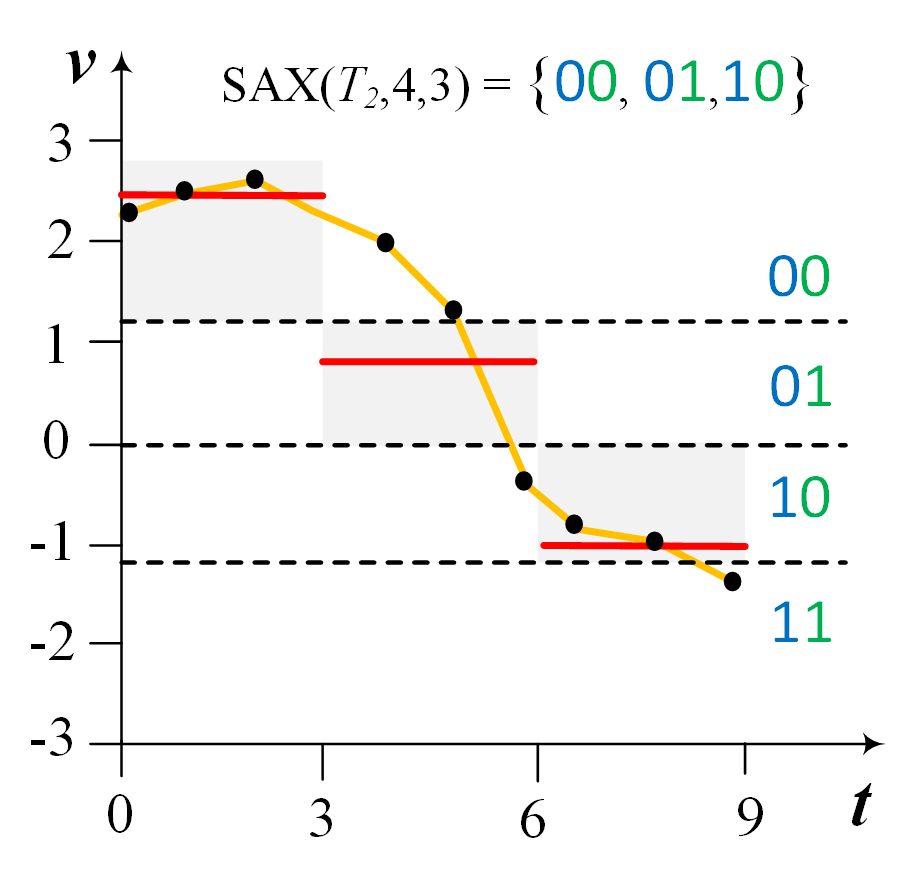
\includegraphics[width=0.5\textwidth]{figures/sax2.pdf}
	\caption{SAX of a time series.}
	\label{fig:isax_representation}
\end{figure}

\subsubsection{The iSAX Family of Indices}
\label{subsec:isax}

Consider the dataset shown in Figure~\ref{fig:sample}. The SAX representation of the time series shown in the example using w=3 words and cardinality 4 is:

\begin{lstlisting}[escapeinside={(*}{*)}]
  	(*$SAX(T_1, 3, 4) = \{00, 01, 11\}$*)
	(*$SAX(T_2, 3, 4) = \{00, 01, 10\}$*)
	(*$SAX(T_3, 3, 4) = \{00, 01, 01\}$*)
	(*$SAX(T_4, 3, 4) = \{10, 01, 01\}$*)
	(*$SAX(T_5, 3, 4) = \{01, 00, 00\}$*)
	(*$SAX(T_6, 3, 4) = \{00, 10, 01\}$*)
	(*$SAX(T_7, 3, 4) = \{01, 00, 00\}$*)
	(*$SAX(T_8, 3, 4) = \{01, 10, 10\}$*)
\end{lstlisting}

By completely ignoring the spatial locations and using the SAX representations of all time series in this dataset, an \isax index \cite{shieh2008kdd} can be built as illustrated in Figure~\ref{fig:isaxtree}. Indeed, the root node captures the complete \isax space and itself does not contain any SAX words, but only points to its children nodes (in the worst case, their number is $2w$). Each leaf has a pointer to a disk file containing the raw time series that represents. The leaf itself also stores the \isax word of highest cardinality among these time series. An internal node designates a split in SAX space and is created when the number of time series contained by a leaf node exceeds a fixed capacity. This split is binary and is made at a given position $j=1..w$ of the SAX word using a round-robin policy, so it always yields two children that differ on their $j$-th symbol while replicating the rest from their parent node. In essence, the SAX space represented by every node fully contains the union of the SAX spaces of its subtree.

\begin{figure}[t]
	\centering
	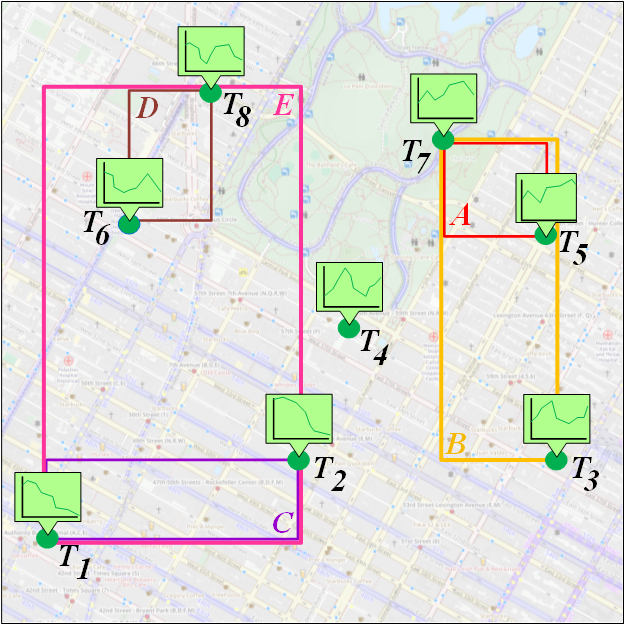
\includegraphics[width=0.5\textwidth]{figures/geoISAX_mbr.png}
	\caption{Sample dataset with MBRs over objects as maintained by the \hisax index}
	\label{fig:sample}
\end{figure}

\begin{figure}[t]
	\centering
	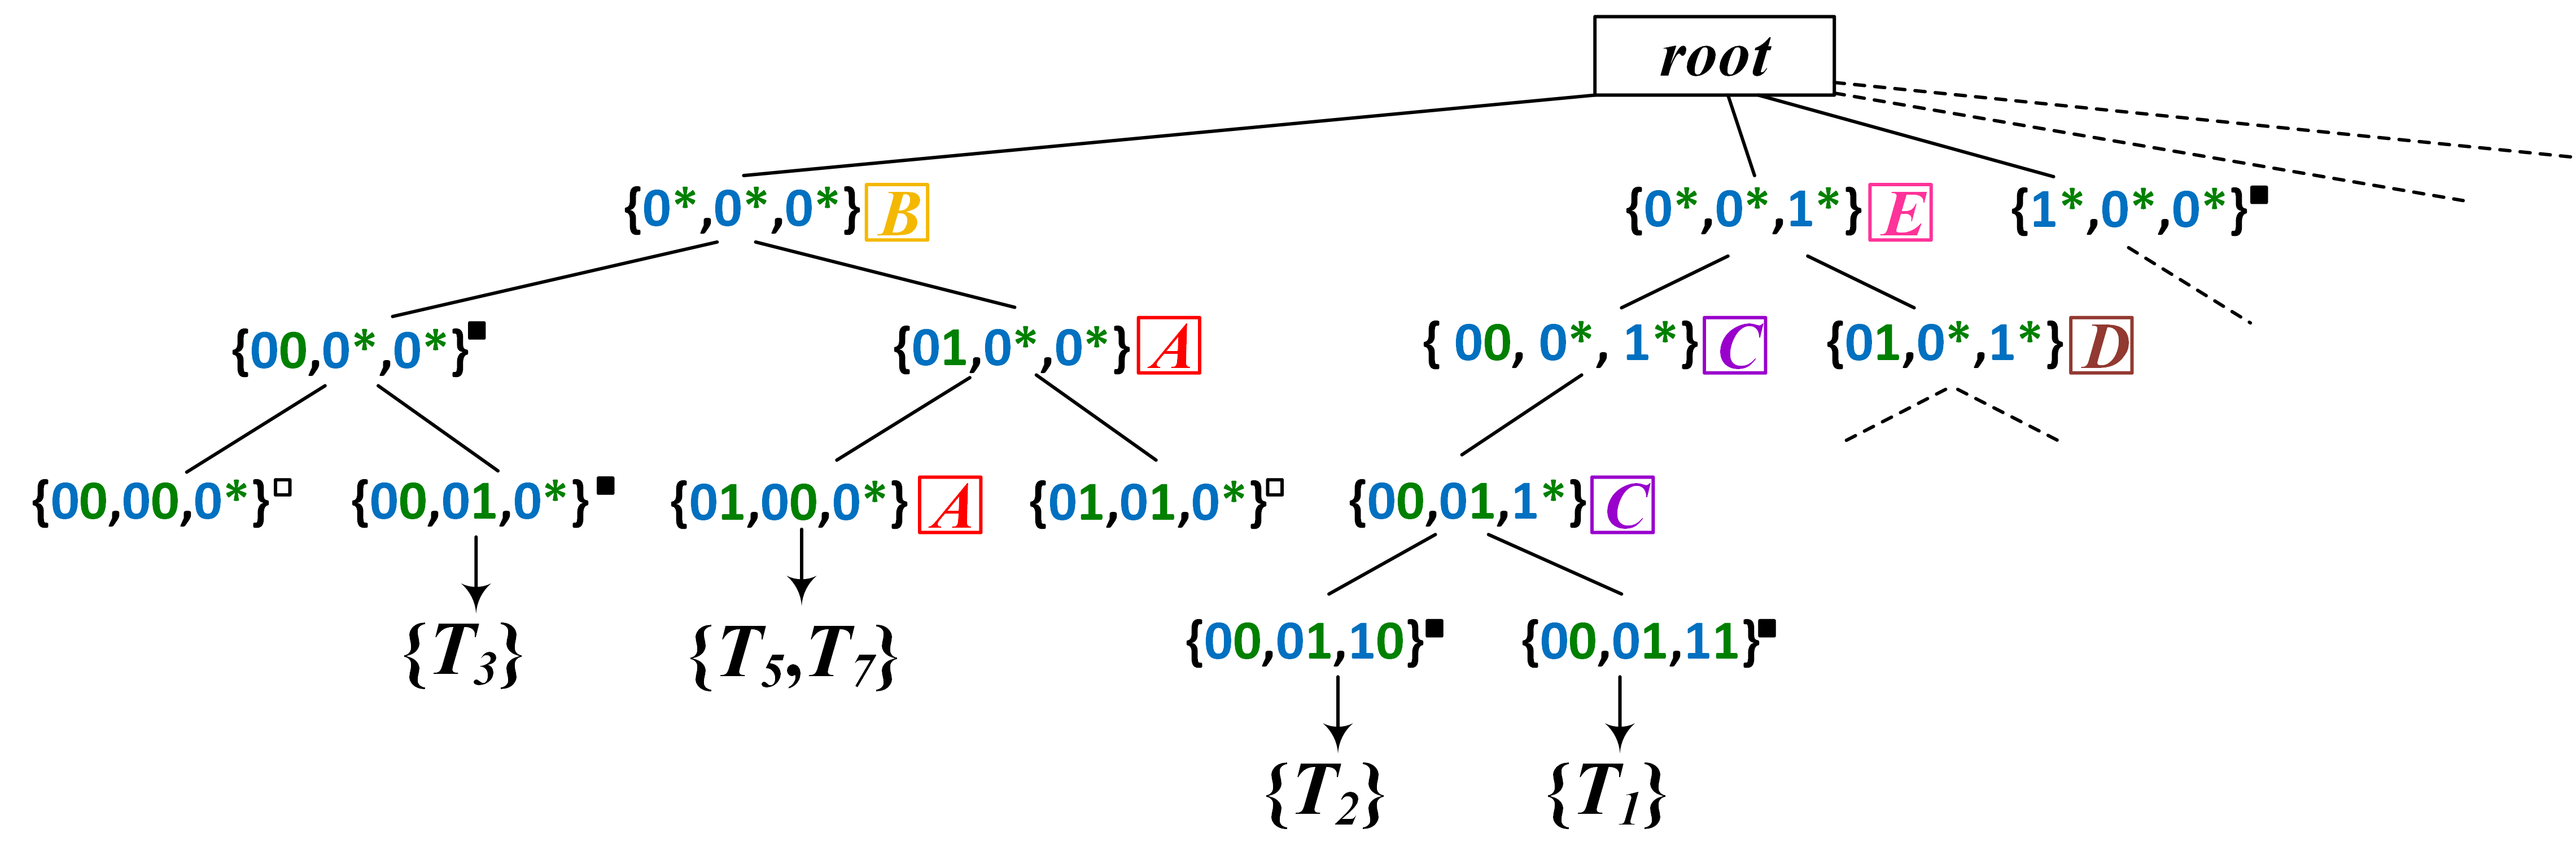
\includegraphics[width=\textwidth]{figures/isax_tree2.pdf}
	\caption{The \hisax index with MBRs attached to each node corresponding to the geolocated time series shown in Figure~\ref{fig:sample}. Nodes with filled boxes indicate a MBR consisting of a single point; nodes with empty boxes indicate no data. Subtrees under dash lines not shown for brevity.}
	\label{fig:isaxtree}
\end{figure}

Searching for time series similar to a query $q$ simply traverses the \isax tree, looking for a leaf node having the same \isax word as query $q$. The respective raw times series are fetched from disk and a sequential scan identifies those matching with $q$. Improvements over the original \isax basically alleviate the bottleneck of expensive I/O when building the index for large datasets; our methodology in Section~\ref{sec:approach} is based on the latest $i$SAX2+ \cite{camerra2014kais}.

\subsection{Minimum Bounding Time Series}
\label{subsec:mbts}

In \cite{chatzig17btsr}, we introduced the notion of {\em Minimum Bounding Time Series} (MBTS), which abstracts {\em a set of time series}  $\mathcal{T}$ using a pair of bounds that fully contain all of them.  Figure~\ref{fig:example_bundle} depicts an example of two MBTSs for two disjoint sets of time series. Formally, given a set of time series $\mathcal{T}$, its MBTS consists of an \emph{upper bounding time series} $T^{\sqcap}$ and a \emph{lower bounding time series} $T^{\sqcup}$, constructed by respectively selecting the maximum and minimum of values at each time point among all time series in set $\mathcal{T}$ as follows:
\begin{align}\label{eq:bounds1}
 \begin{split}
  & T^{\sqcap} = \{ \max_{T \in \mathcal{T}} T.v_1, \ldots, \max_{T \in \mathcal{T}} T.v_{n} \} \\
  & T^{\sqcup} = \{ \min_{T \in \mathcal{T}} T.v_1, \ldots, \min_{T \in \mathcal{T}} T.v_{n} \}
 \end{split}
\end{align}

\begin{figure}[t]
	\centering
	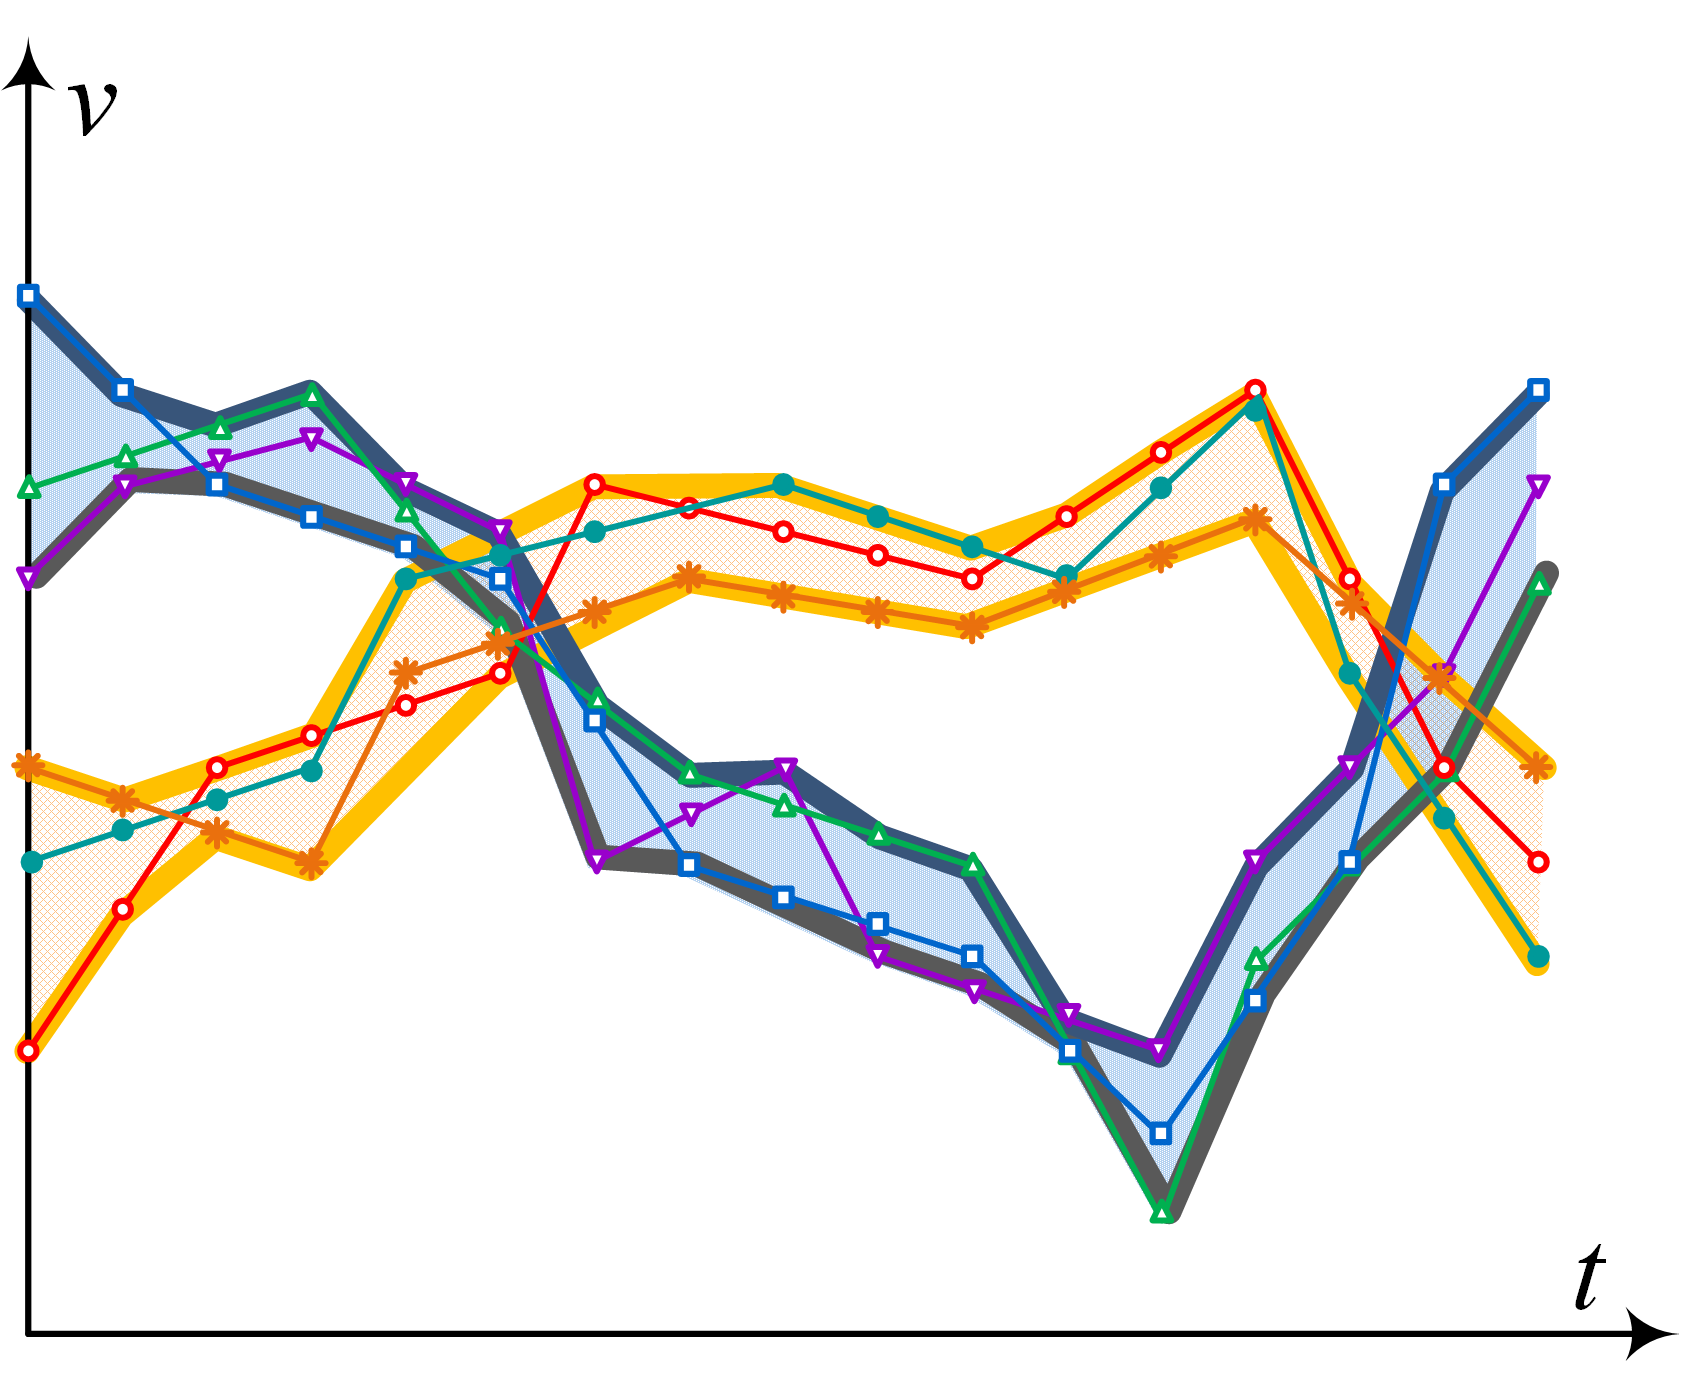
\includegraphics[width=0.5\textwidth]{figures/bounds_btsr.pdf}
	\caption{Example illustrating the resulting bundles for two sets of time series.}
	\label{fig:example_bundle}
\end{figure}

\subsubsection{The \btsr Index}
\label{subsec:btsr}

To efficiently generate real-time visualizations of geolocated time series data, we need early access to both spatial and time series related information while traversing the index, in order to maintain low latency levels when drawing the required graphic elements. However, none of the approaches presented in Section~\ref{sec:related} supports geolocated time series indexing. To the best of our knowledge, the recently proposed \btsr index \cite{chatzig17btsr} is the only one that provides the desired functionality. 

The \btsr is based on the R-tree \cite{Guttman1984} for the spatial indexing part. The R-tree organizes a hierarchy of nested $d$-dimensional rectangles. Each node corresponds to a disk page and represents the MBR of its children or, for leaf nodes, the MBR of its contained geometries. The number of entries per node (excluding the root) is between a lower bound $m$ and a maximum capacity $M$. Query execution in R-trees starts from the root. MBRs in any visited node are tested for intersection against the search region. Qualifying entries are recursively visited until the leaf level or until no further overlaps are found. Several paths may be probed, as multiple sibling entries could overlap with the search region. The \btsr extends the information stored within each node of the R-Tree with bundles of MBTSs. This allows to efficiently prune the search space when evaluating hybrid queries combining time series similarity with spatial proximity.

A \btsr is constructed exactly like an R-tree \cite{Guttman1984} with respect to the spatial contents of a geolocated time series dataset $\mathcal{T}$, as depicted in Figure~\ref{subfig:example}. As in R-trees, each node of the \btsr has at least $m$ and at most $M$ entries and stores the MBRs of its children. Additionally, for each child, a node stores a pre-specified number of MBTSs, shown as colored strips per node in Figure~\ref{subfig:btsrtree}, each one enclosing all the time series indexed in its subtree. Each MBTS is calculated according to Eq.~\ref{eq:bounds1}. Construction and maintenance of the \btsr follow the procedures of the R-tree for data insertion, deletion and node splitting. Objects (i.e., geolocated time series) are inserted into leaf nodes and any resulting changes are propagated upwards. 

Once the nodes have been populated, the MBTS of each node are calculated bottom-up. First, in each leaf node, the contained time series are clustered into $k$ bundles using $k$-{\em means clustering} according to their Euclidean distance in the time series domain. Then, the MBTS of each bundle is computed and stored in the node. The example in Figure~\ref{fig:example_bundle} depicts the $k=2$ MBTSs (as two bands with a thick outline) obtained for a set of time series (shown as thin polylines). As a next step, each parent node receives all the MBTSs of its children and computes its own $k$ bundles and respective set of MBTS by clustering them. The process continues upwards, until reaching the root of the tree. Optionally, \emph{Piecewise Aggregate Approximation} \cite{keogh2001paa,faloutsos2000vldb} can be applied over the time series. As detailed in \cite{chatzig17btsr}, this allows a trade off between the number of bundles per node and the MBTS resolution, thus permitting a larger number ($>k$) of bundles in nodes at higher levels in the tree hierarchy. 

In addition, to support the required functionality of our visualization method, we further extend here the information stored in each node with the {\em count} of geolocated time series that are fully contained within each bundle. This is also done bottom-up, while the index is traversed to calculate the bundles. At each leaf node, after the clustering, we propagate the number of members of each cluster to its parent, which, in turn calculates its clusters and aggregates the counts it has received for each bundle's members. This procedure continues up to the root of the tree.

\begin{figure}[!t]
 \centering
 \subfigure[Spatial-only R-tree index.]{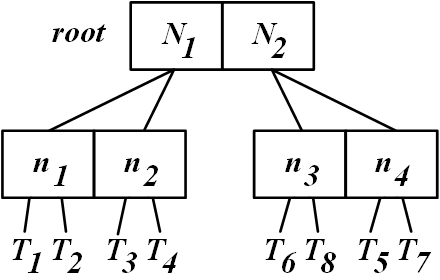
\includegraphics[width=0.45\textwidth]{figures/r_tree.pdf}\label{subfig:example}}
 \subfigure[Hybrid \btsr index..]{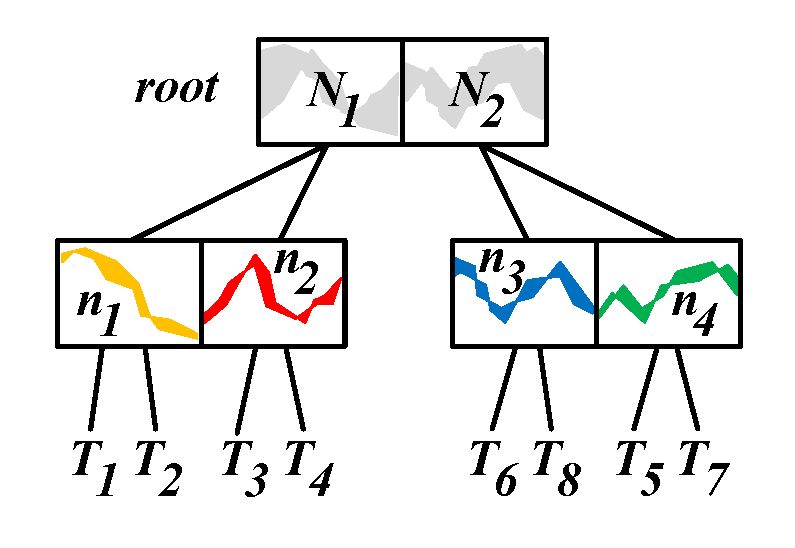
\includegraphics[width=0.45\textwidth]{figures/btsr_tree.pdf}\label{subfig:btsrtree}}\
\caption{The R-tree and \btsr indices.}
\label{fig:trees}
\end{figure}

\subsubsection{Tile Maps} {\em Tile maps} can be used for visually summarizing the concentration of a dataset in a specific domain using rectangle boxes, shaded according to the concentration within each one. They can be used on temporal data to facilitate the detection of patterns or the extraction of useful knowledge regarding the distribution of values in the domain of interest. The higher the concentration of data points within a tile, the darker its shade. We use tile maps in the time series domain, in order to indicate the amount of values that reside within each tile, producing a summary that indicates where the time series of a dataset are concentrated. A tile $b$ is consisted of the following ranges:

\begin{align}\label{eq:tile1}
 \begin{split}
  & b_t = \{t_{min}, t_{max}\} \\
  & b_v = \{v_{min}, v_{max}\}
 \end{split}
\end{align}

\noindent where $\{t_{min}, t_{max}\}$ is a range in the time axis and $\{v_{min}, v_{max}\}$ a range in the value axis. A time series data point $v_x$ is contained in a tile $b$ if:
\begin{align}\label{eq:tile2}
 \begin{split}
  v_x \in b \iff \begin{cases}
  &b.t_{min} \leq x \leq b.t_{max}\\
  &b.v_{min} \leq v_x \leq b.v_{max}
  \end{cases}
 \end{split}
\end{align}

\noindent An example of a tile map for a set of time series is shown in Figure \ref{subfig:tile_map}. The tiles containing more data points are annotated with darker blue shades.

\paragraph{Timebox} A timebox is a rectangular box in the time series domain that fully contains a set of time series in the time and value range that it represents. Essentially, a timebox is an MBR of a time series. Similarly to a tile, a timebox $p$ is consisted of the following ranges:

\begin{align}\label{eq:tb1}
 \begin{split}
  & p_t = \{t_{min}, t_{max}\} \\
  & p_v = \{v_{min}, v_{max}\}
 \end{split}
\end{align}

\noindent where $\{t_{min}, t_{max}\}$ is a range in the time axis and $\{v_{min}, v_{max}\}$ a range in the value axis. A time series $T$ is contained within a time box $B$ if all its data points are contained in it, i.e.:

\begin{equation} \label{eq:tb2}
v_x \in p, \forall v_x \in T
\end{equation}

Figure~\ref{subfig:timebox} depicts with green color, the time series that are contained within a timebox, among a set of time series.